\documentclass[11pt]{article}
%%%%%%%%%%%%%%%%%%%%%%%%%%%%%%%%%%%%%%%%%%%%%%%%%%%%%%%%%%%%%%%%%%%%%%%%%%%%%%%%%%%%%%%%%%%%%%%%%%%%%%%%%%%%%%%%%%%%%%%%%%%%%%%%%%%%%%%%%%%%%%%%%%%%%%%%%%%%%%%%%%%%%%%%%%%%%%%%%%%%%%%%%%%%%%%%%%%%%%%%%%%%%%%%%%%%%%%%%%%%%%%%%%%%%%%%%%%%%%%%%%%%%%%%%%%%
\usepackage{amsfonts}
\usepackage{eurosym}
\usepackage[spanish]{babel}
\usepackage[margin = 0.9in]{geometry}
\usepackage{amsmath,amsthm,amssymb}
\usepackage{graphicx}
\usepackage{comment}
%\usepackage[sort,comma]{natbib}
\usepackage[backend=biber, style = apa]{biblatex}
\usepackage{placeins} % to separate sections

\usepackage{adjustbox}
\usepackage{array}
\usepackage{multirow}
\usepackage{graphicx}
\usepackage{subcaption}
\usepackage{pifont}
\usepackage{amssymb}
\usepackage{comment}
\usepackage[utf8]{inputenc}
\usepackage{setspace}
\usepackage[hang, flushmargin, bottom]{footmisc}
\usepackage{footnotebackref}
\usepackage{xcolor}
\usepackage{hyperref}
\usepackage{booktabs}
\usepackage{pifont}
\usepackage{caption}
\usepackage{float}
\usepackage{todonotes}
\usepackage[normalem]{ulem} % for \sout{} strikethrough
\setcounter{MaxMatrixCols}{10}
%TCIDATA{OutputFilter=LATEX.DLL}
%TCIDATA{Version=5.50.0.2960}
%TCIDATA{<META NAME="SaveForMode" CONTENT="1">}
%TCIDATA{BibliographyScheme=BibTeX}
%TCIDATA{LastRevised=Sunday, April 28, 2024 18:12:38}
%TCIDATA{<META NAME="GraphicsSave" CONTENT="32">}
%TCIDATA{Language=American English}

%\setlength{\bibsep}{0.3pt}
\setlength{\textfloatsep}{5pt}
%\hypersetup{breaklinks=true,hypertexnames=false,colorlinks=true,citecolor = teal}
\captionsetup{font=normalsize}
\newcommand{\cmark}{\ding{51}}
\def\sym#1{\ifmmode^{#1}\else\(^{#1}\)\fi}
\renewcommand{\thetable}{\Roman{table}}
\geometry{verbose,tmargin=.9in,bmargin=1in,lmargin=1in,rmargin=1in,nomarginpar}
\makeatletter
\DeclareTextSymbolDefault{\textquotedbl}{T1}
\theoremstyle{plain}
\newtheorem{thm}{\protect\theoremname}
\theoremstyle{plain}
\newtheorem{prop}[thm]{\protect\propositionname}
\providecommand{\propositionname}{Proposition}
\providecommand{\theoremname}{Theorem}
\makeatother
\providecommand{\propositionname}{Proposition}
\providecommand{\theoremname}{Theorem}
\newtheorem{ass}[thm]{Assumption}
% \input{tcilatex}
\usepackage{tikz}
\usetikzlibrary{shapes.geometric, arrows, positioning}


\usepackage{titlesec}
% 2. Redefine the \section command to use a smaller font size
%    Here we use \large, which is one step smaller than the default \Large.
\titleformat{\section}
  {\normalfont\large\bfseries} % The format for the title (font, size, weight)
  {\thesection}               % The section number
  {1em}                       % The space between the number and title
  {}                          % Optional code before the title text



\addbibresource{../references.bib}
\begin{document}
\spacing{1.2}

 
\title{%{\Large Information sharing policies in financial services}\\
%o\\
{\Large Intercambio de Información y Competencia en Mercados Financieros}}
\author{
Diego Cussen\thanks{Estudiante de doctorado, New York University, \texttt{dc5004@nyu.edu}}
\quad \quad 
Lucas Schmitz\thanks{Estudiante de doctorado, Yale University,  \texttt{lucas.schmitz@yale.edu}}
} 
\date{\today}

\maketitle

\section{Plan de actividades}

\subsection{Propuesta: Motivación, datos y estrategia empírica}


En mercados crediticios, la informacion permite a los bancos predecir el comportamiento de los consumidores. En este contexto, una constante en este tipo de mercado es la asimetria de informacion entre bancos
\footnote{En el mercado de crédito también existen asimetrías de información entre consumidores y bancos, las cuales generan selección adversa; véase, entre otros, \textcite{rothschild_equilibrium_1976}, \textcite{einav_selection_2011} y \textcite{einav_io_2021}. En este documento no nos enfocamos en seleccion adversa, sino que en asimetrías informacionales entre bancos.}.  
En particular, los bancos incumbentes conocen mejor a sus clientes que sus competidores.  Ademas del historial de pago, el banco incumbente observa variables como ingreso, ocupación y demanda por otros productos que el banco ofrece. Esta información adicional le permite estimar con mayor precisión el riesgo crediticio del cliente, y con ello obtener una ventaja informacional. Dicha ventaja informacional genera poder de mercado y distorsiones en la asignación del crédito. 



 
 

\begin{itemize}
    \item Medidas mitigatorias generales%: los gobiernos enfrentan la asimetría de información mediante sistemas de información crediticia. Introducir la ``nómina de deudores'' chilena (Art.\ 14 LGB) como sistema base: bancos, cooperativas y sociedades de apoyo al giro reportan y reciben información consolidada (archivo R04).
\end{itemize}
Para mitigar estas asimetrías, los reguladores establecen sistemas de información crediticia que permiten a los oferentes de crédito compartir datos sobre sus deudores. En Chile, el principal instrumento ha sido la \textit{nómina de deudores} establecida por el artículo 14 de la Ley General de Bancos (DFL~3 de 1997). Bajo este sistema, la CMF mantiene una base de datos consolidada (archivo R04) que agrega la información de deuda reportada por las instituciones financieras fiscalizadas --- cuyo universo ha ido ampliándose con el tiempo. Las entidades que reportan sus deudores son, a su vez, las que reciben la información consolidada, operando bajo un principio de reciprocidad. Este sistema busca reducir la ventaja informacional del acreedor incumbente, permitiendo a sus competidores evaluar mejor el riesgo crediticio de potenciales clientes.

\begin{itemize}
    \item Historial cronológico de políticas chilenas%: (a) Leyes 20.455/20.522/20.575 (2010--2012) eliminan información de deudores del sistema; (b) Ley 21.130 (2019, implementada 2021--22) incorpora emisores de tarjetas no bancarios (ETNB); (c) Ley 21.680 REDEC (2024, vigente abril 2026) amplía a OCNB, compañías de seguro, cajas, securitizadoras, e incluye info positiva; (d) Ley Fintec (2023) establece banca abierta vía APIs.
\end{itemize}   

El marco regulatorio chileno en materia de información crediticia ha experimentado múltiples reformas en los últimos quince años. Entre 2010 y 2012, tres leyes sucesivas (Leyes 20.455, 20.522 y 20.575) \textit{restringieron} la información disponible en el sistema, eliminando registros de morosidad para desempleados de corto plazo, excluyendo consultas crediticias del puntaje, y borrando historiales de impago por montos menores a aproximadamente \$1.500 USD, lo cual afectó a 2,8 millones de personas \parencite{liberman_equilibrium_2018, madeira_impact_2024}. En dirección opuesta, la Ley 21.130 de modernización bancaria \textit{amplió} el sistema entre 2021 y 2022 al incorporar a los emisores de tarjetas de crédito no bancarios (ETNB) como reportantes y receptores de la nómina de deudores. Más recientemente, la Ley 21.680, que crea el Registro de Deuda Consolidada (REDEC) y entra en vigencia el 1 de abril de 2026, expande significativamente el universo de entidades que participan del sistema informacional. Finalmente, la Ley Fintec (Ley 21.521) establece un sistema de finanzas abiertas que, una vez implementado, permitirá el intercambio de datos financieros entre instituciones mediante APIs estandarizadas.
\begin{itemize}
    \item Descripcion REDEC: %expande de $\sim$4 a $\sim$10+ tipos de entidades reportantes; incorpora información positiva (no solo morosidad); requiere consentimiento previo del deudor para consultas. La novedad clave: oferentes de crédito no bancarios (cajas de compensación, compañías de seguro, securitizadoras, asesores crediticios Fintec) entran al sistema por primera vez.
\end{itemize} 
% --- New Version ---
El REDEC amplía sustancialmente el universo de entidades que participan del sistema de información crediticia. Bajo el sistema anterior del artículo 14 LGB, solo las instituciones financieras fiscalizadas reportaban y recibían información consolidada. El REDEC extiende esta obligación a oferentes de crédito no bancarios (OCNB), incluyendo cajas de compensación y compañías de seguro, entre otros.\footnote{La lista completa de entidades reportantes se establece en el artículo 2, letra e) de la Ley 21.680. Además de cajas de compensación y compañías de seguro, incluye agentes administradores de mutuos hipotecarios endosables, sociedades securitizadoras, asesores crediticios regulados por la Ley Fintec, y acreedores no fiscalizados que superen ciertos umbrales de actividad.} En cuanto al contenido, el REDEC incorpora información positiva --- es decir, datos sobre el comportamiento de pago y las condiciones de los créditos vigentes --- y no solamente datos de morosidad, como ocurría en el sistema previo.

\begin{itemize}
    \item Contexto internacional:% la expansión de registros crediticios públicos es una tendencia global. Mencionar ejemplos comparables. Esto da validez externa al estudio del REDEC.
\end{itemize} 
% --- New Version ---
Una manifestación destacada de las reformas regulatorias orientadas a reducir asimetrías de información en mercados financieros son las leyes de finanzas abiertas (\textit{open finance}), que establecen mecanismos para el intercambio estandarizado de datos financieros entre instituciones. Estas regulaciones están siendo adoptadas en un número creciente de países. En Europa, la Directiva de Servicios de Pago (PSD2) y las regulaciones de banca abierta en el Reino Unido sentaron precedentes que han sido emulados en América Latina, donde Brasil\footnote{\url{https://www.bcb.gov.br/en/financialstability/open_finance}}, México\footnote{\url{https://www.hklaw.com/en/insights/publications/2020/07/open-banking-has-arrived-in-mexico}} y Colombia\footnote{\url{https://www.hklaw.com/en/insights/publications/2022/08/conozca-los-aspectos-relevantes-de-la-regulacion-sobre-finanzas}} han avanzado en la misma dirección. El REDEC, junto con la Ley Fintec, sitúa a Chile dentro de esta tendencia. Dado que estas reformas se están implementando en múltiples países de manera simultánea, generar evidencia rigurosa sobre sus efectos es particularmente relevante para orientar el diseño de políticas regulatorias tanto en Chile como en la región.



\begin{itemize}
    \item Tensiones en la dirección de política: el historial chileno muestra políticas en direcciones opuestas---algunas eliminan información (leyes 2010--12), otras la amplían (Ley 21.130, REDEC, Fintec). Esta ambigüedad demanda evidencia empírica rigurosa sobre los efectos de compartir más información.
\end{itemize} 
% --- New Version (Tensiones) ---
Como se desprende del recuento anterior, las políticas chilenas en materia de información crediticia han respondido a diversos objetivos. Las leyes de 2010--2012 buscaron proteger a los deudores vulnerables restringiendo la información disponible en el sistema, mientras que las reformas posteriores --- Ley 21.130, REDEC y Ley Fintec --- buscan promover la competencia y mejorar la asignación del crédito ampliando el intercambio de información. La evidencia empírica disponible sugiere que las múltiples fuerzas en juego pueden operar en distintas direcciones: \textcite{madeira_impact_2024} muestra que la eliminación focalizada de información (Ley 20.455 de 2010) mejoró el acceso al crédito, mientras que la eliminación masiva (Ley 20.575 de 2012) tuvo el efecto contrario; por su parte, \textcite{foley_effects_2020} documentan que compartir más información aumenta la competencia por buenos deudores pero puede perjudicar la inclusión financiera. Cuantificar la magnitud relativa de estas fuerzas es esencial para evaluar los efectos del REDEC.



\begin{itemize}
    \item Fuerzas teóricas %: Sharpe (1990), Petersen \& Rajan (1995), Dell'Ariccia et al.---más información reduce rentas informacionales y baja tasas para buenos deudores, pero puede generar \textit{cream-skimming} y excluir a deudores riesgosos o nuevos. Efecto específico del REDEC: deudores de OCNB que eran ``invisibles'' para bancos ahora se vuelven observables.

% --- New Version ---
La literatura teórica identifica fuerzas contrapuestas asociadas al intercambio de información crediticia. Por un lado, cuando la información sobre la calidad de los deudores se vuelve pública, la ventaja informacional del acreedor incumbente se reduce, lo que intensifica la competencia y disminuye las tasas de interés para los deudores de bajo riesgo \parencite{sharpe_asymmetric_1990, petersen_effect_1995}. Además, al reducirse la asimetría de información entre acreedores, disminuye la selección adversa que enfrentan los competidores del incumbente, facilitando la entrada de nuevos oferentes al mercado. Por otro lado, la pérdida de rentas informacionales puede reducir el acceso al crédito de clientes nuevos o sin historial. La intuición es la siguiente: en un régimen sin intercambio de información, el acreedor que invierte en conocer a un cliente nuevo puede recuperar esa inversión en el futuro, cobrándole tasas superiores a las competitivas gracias a su ventaja informacional. Si esa ventaja desaparece porque la información se comparte, el retorno esperado de otorgar crédito a clientes desconocidos cae, y con ello el incentivo a hacerlo \parencite{petersen_effect_1995, dellariccia_information_2004}. En el contexto específico del REDEC, los deudores de oferentes de crédito no bancarios (OCNB) --- históricamente ``invisibles'' para los bancos --- se vuelven observables. Esto beneficia a los buenos deudores de OCNB, que ahora estarán expuestos a ofertas competitivas de bancos; pero la reducción de las rentas informacionales de los OCNB puede disminuir los incentivos de estos para otorgar crédito a nuevos clientes.


    \item Pregunta de investigación: ¿Cómo afecta la ampliación del reporte de información crediticia a oferentes no bancarios (REDEC) la competencia, asignación del crédito, tasas de interés e inclusión financiera?

% --- New Version ---
La presencia de potenciales efectos adversos en los clientes entrantes provoca que el  impacto neto de la BA sobre el bienestar sea incierto. 
En este contexto, el presente proyecto busca responder la siguiente pregunta: \textbf{¿cómo afecta el REDEC (Ley 21.680) el equilibrio en el mercado crediticio? con un especial enfasis en los efectos heterogeneos que puede tener en distintos grupos de la poblacion. Como puede ser la reduccion al acceso al credito de individuos sin historial previo en el sistema. }



    \item Relevancia institucional %para la CMF: vincular directamente con el mandato del Art.\ 1 Ley 21.000 (estabilidad, desarrollo del mercado, protección de consumidores). Además, mayor competencia afecta el \textit{pass-through} de política monetaria, relevante para la estabilidad financiera.
    
Esta investigación está directamente alineada con el mandato institucional de la CMF. El artículo 1 de la Ley 21.000 encarga a la Comisión ``velar por el correcto funcionamiento, desarrollo y estabilidad del mercado financiero, facilitando la participación de los agentes de mercado y promoviendo el cuidado de la fe pública''. Nuestro proyecto contribuye a este mandato en dos dimensiones. Primero, al estudiar si el REDEC intensifica la competencia y reduce las tasas para deudores de bajo riesgo, generamos evidencia directa sobre si la reforma cumple su objetivo de promover el \textit{desarrollo} del mercado financiero. Segundo, al evaluar si la reforma reduce el acceso al crédito de nuevos entrantes, informamos sobre potenciales riesgos para la \textit{inclusión financiera}.


\end{itemize}





%\begin{figure}[!ht]
%    \centering
%    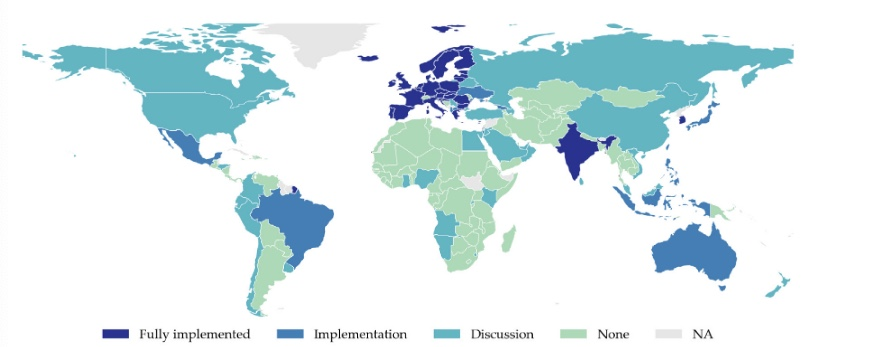
\includegraphics[width=0.8\linewidth]{../figures/Screenshots/map_babina2.jpeg}
%    \caption{Banca abierta en el mundo en 2021. \textit{Fuente}: \textcite{babina_customer_2025}.}
%    \label{fig:map_babina2}
%\end{figure}



 





En lo que sigue, detallaremos tanto los datos necesarios como los desafíos y enfoque empírico utilizado para responder a nuestra pregunta de investigación.

\newpage






\paragraph{Desafios empiricos}

Dos desafíos dificultan hacer investigación sobre los efectos de la banca abierta. El primero es que los bancos e instituciones financieras anticipan la entrada en vigor de las reformas que implementan la BA.
En este caso, uno esperaria que los efectos negativos en los clientes entrantes deberian comenzar a observarse antes de la implementacion de la BA, pues los bancos ya saben que el retorno de obtener más información va a caer significativamente en un futuro cercano. 

Luego, estrategias empíricas que utilizan la fecha de implementación de una reforma para identificar sus efectos (como diferencias endiferencias o estudio de eventos) no pueden capturar todos los efectos de la BA.\footnote{Este problema ya fue demostrado en el caso del efecto de la integración del Sistema Interconectado Norte y el Sistema Interconectado Central sobre la inversión en paneles solares en Chile (\cite{gonzales_investment_2023}).} En Chile, donde la Ley Fintec se aprobó en 2023 pero entrará en vigencia en 2026, es de esperar que estos efectos anticipatorios estén presentes.

El segundo desafío concierne a la calidad de los datos. Para estudiar el impacto de la BA en los distintos segmentos de la población necesitamos seguir a los clientes en el tiempo y entre bancos. Ademas, para estudiar la inclusión financiera, es útil observar no solo los créditos entregados sino que también las aplicaciones no exitosas, casos en los que un cliente solicita un crédito pero el banco lo rechaza. Si uno no observa el universo de aplicaciones es difícil determinar si un resultado de equilibrio (ej. bajo nivel de endeudamiento) es resultado de fuerzas de demanda (ej. individuos no solicitan crédito) o fuerzas de oferta (ej. bancos rechazan aplicaciones).  

El contexto chileno tiene características que permiten solventar los dos desafíos mencionados previamente, lo que lo convierte en el escenario ideal para estudiar los impactos de la BA. 
Primero, la entrada en vigencia de la BA será escalonada, ya que la Ley Fintec se implementara en forma progresiva para  distintas instituciones, clientes y tipos de información.\footnote{Por ejemplo, la obligación de compartir posiciones financieras históricas entraría en vigor para personas naturales tres meses antes que para personas jurídicas. \url{https://www.cmfchile.cl/portal/prensa/615/w3-article-82737.html}.} Incluso si hay efectos anticipatorios, la entrada en vigor escalonada permite identificar, al menos parcialmente, efectos diferenciales de acceso a información sobre distintos tipos de prestatarios. Segundo, la calidad de los datos chilenos es muy alta. Específicamente, la CMF cuenta con datos que permiten dar seguimiento a individuos a lo largo del tiempo y entre diferentes bancos, incluyendo no solo los créditos que los individuos adquieren, sino que también las aplicaciones rechazadas. 


 

\paragraph{Datos solicitados}


Para materializar esta investigación, 
los datos de alta frecuencia que requerimos de la Comisión para el Mercado Financiero (CMF) serían los siguientes:


\begin{itemize}
    \item Datos individuales de deudores sobre:
    \begin{itemize}
        \item Tarjetas de crédito bancarias y no bancarias: uso, pago y morosidad
        \item Préstamos individuales: montos, tasas de interés, planes de pago, vencimientos y morosidad
        \item Cuentas individuales (vista, corriente y de ahorro): saldos y movimientos
        \item Créditos hipotecarios: montos, tasas de interés, planes de pago, vencimientos y morosidad (hablar en lit review que Allen et al muestran la importancia del home bank. creemos que la hipoteca (y cambios en el banco acreedor de la hipoteca) es una forma útil de determinar cuál es el home bank
    \end{itemize}
    \item Datos sobre postulaciones a préstamos, exitosas y fallidas.
\end{itemize}


Esta investigación está alineada con el mandato legal de la CMF, en particular, su rol de velar por la protección de los clientes y depositantes y promover el desarrollo del mercado financiero. 


 

\paragraph{Estrategia empirica}

Empiricamente nuestra investigación consta de dos partes. La primera parte presenta evidencia en forma reducida de los impactos de BA. La segunda parte consiste en un modelo económico (para fijar ideas) que guía la interpretación de los efectos de equilibrio del mercado.

Hay dos razones por las que la evidencia en forma reducida no es suficiente para estudiar el impacto de la reforma. Primero, como ya mencionamos previamente, dado que los bancos anticipan la reforma, al estimar un modelo en forma reducida, podríamos encontrar un efecto nulo  de la reforma incuso en el caso de que si haya un efecto. La segunda razón es que hay efectos de equilibrio general. Por ejemplo, \textbf{... HAY EFECTOS DE EQ GENERAL? NO ESTOY SEGURO}. A continuación presentamos nuestra estrategia empírica para obtener resultados en forma reducida. 

El primer paso consiste en establecer una relación empírica entre la implementación de la BA y el acceso al crédito de los individuos con un perfil de crédito favorable. Para eso utilizamos un estudio de eventos\footnote{Para una introducción a los estudios de eventos ver \textcite{miller_introductory_2023}.},  que nos permite usar la variación en la entrada en vigor de la Ley Fintec para estimar sus efectos en el mercado financiero. Las dos especificaciones que estimamos son: 
%El primer paso para identificar los efectos de la BA es establecer una relación empírica entre la implementación de la BA y la competencia en el mercado financiero y acceso a crédito en Chile. Para eso utilizamos un estudio de eventos\footnote{Para una introducción a los estudios de eventos ver \textcite{miller_introductory_2023}.},  que nos permite usar la variación en la entrada en vigor de la Ley Fintec para estimar sus efectos en el mercado financiero. La principal ecuación a estimar es:
\begin{equation}
    \Pr(y_{it}=y_{it}^P|y_{it} > 0, H_{it}= N) = f\left( 
    \underbrace{\sum_{j\in \{-m,..., 0,...,n\}}\gamma_j D_{i,t-j}}_{\text{Estudio de eventos}} +
    \underbrace{\alpha_i 
    %+ \delta_t
    }_{\text{Efectos fijos}} +
    \underbrace{\beta x_{it}}_{\text{Controles}} + e_{it}\right) 
    \label{eqn:main_linear_model}
\end{equation}

\begin{equation}
    r_{it} = 
    \underbrace{\sum_{j\in \{-m,..., 0,...,n\}}\gamma_j^r D_{i,t-j}}_{\text{Estudio de eventos}} +
    \underbrace{\alpha_i^r 
    %+ \delta_t
    }_{\text{Efectos fijos}} +
    \underbrace{\beta^r x_{it}}_{\text{Controles}} + e_{it}^r 
    \label{eqn:main_linear_model2}
\end{equation}

Las ecuaciones \ref{eqn:main_linear_model} y \ref{eqn:main_linear_model2} serán estimadas en la población de individuos con un buen historial crediticio. \footnote{Para clasificar a los individuos en términos de su historial crediticio podríamos usar técnicas de \textit{machine learning} siguiendo a \textcite{liberman_equilibrium_2018}. }
La ecuación \ref{eqn:main_linear_model} busca estimar el efecto de la BA en el tasa movilidad de clientes con un buen historial. La ecuación \ref{eqn:main_linear_model2} busca estimar el efecto de la BA en las tasas de interés a las cuales los clientes con buen historial se endeudan.

A continuación detallamos la notación usada. El sub-indice $i$ indexa individuos y $t$ indexa periodo de tiempo, por ejemplo mes. Los otros términos son: 

\begin{itemize}
    \item $y_{it} \in \{0, 1, ..., N\}$ representa institución bancaria en la cual el individuo obtiene un crédito, donde $y_{it} = 0$ indica que el individuo no obtuvo un crédito en dicho periodo, e $y_{it} = b>0$ significa que obtuvo un crédito del banco indexado con el numeral $b$. 
    \item $y_{it}^P$ representa el ultimo banco del cual el individuo obtuvo un crédito. Formalmente 
    
    $$y_{it}^P =  \begin{cases}
        y_{it^-}\quad,  \text{si} \  t^- = \max\{s<t: y_{is}>0\} \ \text{existe} \\
        \emptyset \quad \quad , \text{si no hay historial previo}
    \end{cases}$$ 
    
    \item $H_{it}\in \{\emptyset, R, NR\}$ representa el historial crediticio del individuo. Donde $H_{it} =\emptyset$ indica que el individuo no tiene historial crediticio, $H_{it}= R$ indica que tiene un historial de impagos lo que implica que es un cliente riesgoso y $H_{it}= NR$ indica que en base a su historial es un cliente no riesgoso. Para clasificar a los individuos podríamos usar técnicas de \textit{machine learning} siguiendo \textcite{liberman_equilibrium_2018}.  
    
    \item $D_{i, t-j}$ es una variable indicadora que toma el valor 1 si la politica de BA fue implementada $j$ periodos previo a $t$. Por lo que los coeficientes $\gamma_j$ capturan los efectos del tratamiento a lo largo del tiempo. 

    \item $\alpha_i$ nos permiten capturar efectos individuales persistentes en el tiempo, por ejemplo que ciertos individuos tienen menores costos de búsqueda lo que genera un mayor \textit{switching rate}.

    \item $x_{it}$ son controles, que dependen de los datos a los cuales tengamos acceso, ellos permiten aislar efectos a nivel individual que son variables en el tiempo, por ejemplo el impacto de un aumento de los ingresos laborales del individuos o el impacto de la edad en el \textit{switching rate}. 

    \item $f(x) = \exp(x)/(\exp(x) +1)$ es la función logística.
\end{itemize}

 
Los coeficientes de interés en la ecuación \ref{eqn:main_linear_model} son los $\gamma_j$ y en \ref{eqn:main_linear_model2} son los $\gamma_j^r$. Los coeficientes correspondientes a periodos posteriores a la implementación de la ley ($\gamma_j,  \gamma_j^r$ para $j \geq 0$) capturan los efectos de la BA, que pueden variar en el tiempo. La teoría previamente presentada predice que los $\gamma_j$ post-implementación sean positivos y que los $\gamma_j^r$ post-implementación sean negativos. Los coeficientes correspondientes a periodos previos a la implementación ($\gamma_j,  \gamma_j^r$ para $j < 0$) proveen un test placebo, por lo que esperaríamos que no fueran estadisticamente significativos. 


%donde $y_{it}$ es una variable de resultado para un agente $i$ en periodo $t$, donde el periodo es relativo al mes en que la BA comenzó a afectar a ese agente. \textbf{explicar timing, controles, efectos fijos, residuo. tal vez buena idea explicar tendencias diferenciales, como caronine.}


 

Como se explicó antes, en presencia de efectos anticipativos no es posible estimar el impacto de la reforma en los clientes entrantes. 
Por eso, el segundo paso es construir un modelo en que bancons compiten por otorgar créditos a clientes con distinta capacidad de pago. En un régimen sin BA, un banco con quien el cliente ya tiene una relación posee una ventaja informacional, pues es el único con datos detallados sobre la capacidad de pago del cliente. Con BA esta ventaja desaparece. Los bancos otorgan créditos repetidamente en el tiempo, sabiendo que la BA se implementará en el futuro. Usando los datos de la CMF antes, durante y después de la implementación de la ley Fintec, es posible estimar los parámetros que gobiernan el comportamiento de bancos y clientes. Estas estimaciones permiten estudiar en detalle los efectos de la BA incluso si los bancos anticipan la reforma, incluyendo sus efectos distributivos y sobre el bienestar de la población. Para fijar ideas, en el Anexo a este documento incluimos un modelo simplificado de este tipo.

 


%Como se explicó antes, en presencia de efectos anticipativos se espera que una ecuación como (\ref{eqn:main_linear_model}) sea incapaz de capturar completamente los efectos de la BA. Por eso, el segundo paso es construir un modelo en que bancons compiten por otorgar créditos a clientes con distinta capacidad de pago. En un régimen sin BA, un banco con quien el cliente ya tiene una relación posee una ventaja informacional, pues es el único con datos detallados sobre la capacidad de pago del cliente. Con BA esta ventaja desaparece. Los bancos otorgan créditos repetidamente en el tiempo, sabiendo que la BA se implementará en el futuro. Usando los datos de la CMF antes, durante y después de la implementación de la ley Fintec, es posible estimar los parámetros que gobiernan el comportamiento de bancos y clientes. Estas estimaciones permiten estudiar en detalle los efectos de la BA incluso si los bancos anticipan la reforma, incluyendo sus efectos distributivos y sobre el bienestar de la población. Para fijar ideas, en el apéndice a este documento incluimos un modelo simplificado de este tipo. 

\vspace{2cm} 


La primera contribución de este trabajo es un test empírico detallado de las teorías sobre los efectos de la información asimétrica en el mercado financiero. \textcite{sharpe_asymmetric_1990}, \textcite{petersen_effect_1995}, \textcite{dellariccia_adverse_1999} y \textcite{dellariccia_information_2004} notan que los efectos positivos de la competencia en el mercado financiero dependen de la extensión del problema de información asimétrica.

En el ámbito empírico, artículos relacionados son \textcite{petersen_benefits_1994,petersen_effect_1995}, \textcite{liberman_equilibrium_2018} y \textcite{foley_effects_2022}. El artículo más relacionado al presente trabajo es \textcite{foley_effects_2022}, que estudia la adquisición, en Chile, de un proveedor no bancario de tarjetas de crédito por parte de un banco. Esta adquisición fue una sorpresa, por lo que constituye un experimento natural. 

Al pasar a la cartera del banco, información sobre los clientes del prestamista no bancario (``el prestamista'') se volvió observable para otros bancos, aumentando la competencia por otorgar crédito a los clientes de ``buen tipo'' (alta acapcidad de repago) del prestamista. El costo es el riesgo de excluir a los prestatariosn más riesgosos, tal como predice la teoría. Crucialmente, los autores no encuentran que aumentar la información disponible resulte en mayor colusión -- un riesgo conocido en la literatura de organización industrial.\footnote{Papers de \textcite{green_noncooperative_1984}, Montag et al?, y Cussen and Montero (2024).}

Nuestro trabajo va significatimvemente más allá que \textcite{foley_effects_2022}. Primero, el cambio en el régimen informacional causado por la Ley Fintec afectará a todas las empresas y consumidores, creando efectos de equilibrio general que son difíciles o imposibles de capturar usando diferencia-en-diferencias. Por ejemplo, el experimento natural estudiado por \textcite{foley_effects_2022} solo aumenta la información de un subconjunto de empresas en el mercado (bancos) sobre una empresa de otro subconjunto (prestamistas no bancarios). La SFA haría pública toda la información, así que los bancos tendrían más información sobre los clientes de otros bancos, etc. ponerle color. 

Segundo, la Ley Fintec se aprobó años antes de su entrada en vigor. Luego, su efecto no puede medirse a partir del moemnto de su entrada en vigor, pues a ese momento los bancos ya habrán ajustado su comportamiento en cuanto a préstamos a nuevos clientes, y los clientes también pueden haber ajustado su probabilidad de repago, pues saben que serán observados por el resto del sistema financiero pronto.\footnote{Ver Pagano and Jappelli (1993), Padilla and Pagano (1997,200), citados en \textcite{foley_effects_2022}.} Las conisderaciones de este párrafo y el anterior llevan a concluir que una evaluación del efecto be implementar un SFA require un modelo estructural, como proponemos.

Finalmente, el uso de un modelo estrucutural nos permite medir los efectos distributivos y sobre el bienestar de un SFA y de políticas alternativas.

%\textcite{foley_effects_2020} estudian el efecto de la adquisición de un proveedor no bancario de tarjetas de crédito en Chile por parte de un banco. Al pasar a la cartera del banco, información sobre los clientes del prestamista no bancario se vuelve observable por otros bancos, lo que aumenta la competencia por otorgarles créditos. Los autores muestran que la competencia aumenta la eficiencia asignación de crédito entre clientes con capacidad de repago, a riesgo de excluir prestatarios más riesgosos del mercado. \textbf{EXPLICAR QUE EN FOLEY SOLO UNA EMPRESA CAMBIA DE REGIMEN, ENTOCNES NO PUEDE ESTIMAR EFECTOS DE EQUILIBRIO QUE SE DAN CUANDO TODAS LAS EMPRESAS CAMBIAN DE REGIMEN.} 

Tercero, este trabajo contribuye a una reciente literatura que estudia los impactos de la competencia en mercados con informacion asimetrica; ver \textcite{allen_search_2019}, \textcite{cuesta_price_2018} y \textcite{cosconati_competing_2025}. 



    \newpage
    \section*{Modelo de informacion asimetrica}
    {\small

    Este anexo resume el modelo  usado para formalizar cómo la asimetría informacional entre bancos y los costos de cambio (\textit{switching costs}) interactúan para determinar tasas de equilibrio, asignación de crédito e inclusión financiera.

    \paragraph{Juego en dos etapas (intuición)}
    \begin{enumerate}
        \item \textbf{Etapa 1 (producto introductorio).} Dos bancos compiten por captar al consumidor con un producto inicial (p.ej., cuenta corriente, tarjeta). Ex ante ninguno conoce el riesgo del consumidor.
        \item El banco elegido pasa a ser el \textbf{banco incumbente (\textit{home bank})} y observa información adicional durante la relación, aprendiendo el tipo $h$ del consumidor (probabilidad de default). El otro banco queda como \textbf{entrante no informado}.
        \item \textbf{Etapa 2 (mercado de crédito).} Ambos bancos compiten por otorgar un crédito. Si el consumidor se cambia al banco entrante, incurre un costo de cambio $\lambda\ge 0$.
    \end{enumerate}

    \paragraph{Etapa 2: demanda y utilidades}
    Una especificación estándar (logit) para la utilidad indirecta de endeudarse con el banco $j\in\{1,2\}$ es:
    \begin{align*}
        u_{1} &= -\alpha\, r_{1} + \varepsilon_{1}\\
        u_{2} &= -\alpha\, r_{2} - \lambda + \varepsilon_{2}
    \end{align*}
    donde $r_j$ es la tasa, $\alpha>0$ captura sensibilidad al precio y $(\varepsilon_1,\varepsilon_2)$ son shocks de preferencia. La probabilidad de elegir al incumbente es
    \begin{align*}
        s(r_1,r_2) = \frac{1}{1+\exp\!\big(\alpha(r_1-r_2)-\lambda\big)}.
    \end{align*}

    \paragraph{Etapa 2: costos, tipos y beneficios}
    El tipo $h\in(0,1)$ es la probabilidad de default. Con costo de fondeo normalizado a 1 por préstamo, la tasa de equilibrio de punto de quiebre para un tipo $h$ es $c(h)=\tfrac{1}{1-h}$. La ganancia esperada por préstamo (margen) es $(1-h)r-1$.

    El incumbente observa $h$ y puede fijar una tasa dependiente del tipo, $r_1=\sigma(h)$. El entrante no observa $h$ y fija una única tasa $r_2$.

    \paragraph{Etapa 2: caracterización de equilibrio (idea central)}
    En equilibrio, el banco informado fija (para cada tipo) una tasa igual a \textbf{break-even + markup}:
    \begin{align*}
        \sigma^*(h) = \frac{1}{1-h} + \underbrace{m_1\big(\sigma^*(h),r_2^*\big)}_{\text{markup}}.
    \end{align*}
    Bajo logit, el markup toma forma cerrada en función de la participación $s$:
    \begin{align*}
        \sigma^*(h) = \frac{1}{1-h} + \frac{1}{\alpha\big(1-s(\sigma^*(h),r_2^*)\big)}.
    \end{align*}
    El banco no informado elige $r_2^*$ maximizando su beneficio agregado (integrando sobre $h$), lo que genera una condición de primer orden que equivale a una regla de \textbf{break-even + markup promedio ponderado}. En el modelo, esto produce \textit{cream-skimming}: el incumbente retiene relativamente más a los tipos seguros y el entrante enfrenta una cartera adversamente seleccionada.

    \paragraph{Etapa 1: inducción hacia atrás y \textit{loss-leading}}
    La solución de etapa 2 determina el valor de ser incumbente (informado) versus entrante (no informado):
    \begin{align*}
        V^{I} &= \int \big[(1-h)\,\sigma^*(h)-1\big]\, s\big(\sigma^*(h),r_2^*\big)\, dF(h),\\
        V^{E} &= \int \big[(1-h)\,r_2^*-1\big]\, \big[1-s\big(\sigma^*(h),r_2^*\big)\big] \, dF(h),\\
        \Delta V &= V^{I}-V^{E}.
    \end{align*}
    Al competir en etapa 1 por captar al cliente, cada banco está dispuesto a sacrificar hasta $\Delta V$ en el precio del producto introductorio. Esto racionaliza \textbf{precios iniciales bajos (incluso bajo costo)} y, al mismo tiempo, \textbf{tasas más altas} en la etapa 2 por la interacción entre ventaja informacional y costos de cambio.

    }









\newpage
\printbibliography
 
\subsection{Graficos}
\end{document}
